%%%%%%%%%%%%%%%%%%%%%%%%%%%%%%%%%%%%%%%%%%%%%%%%%%%%%%%%%%%%%%%%%%%%%%%%%%
% DisplayOfCurrentsAndVoltagesDependingOnTheSwitchingPhases
%%%%%%%%%%%%%%%%%%%%%%%%%%%%%%%%%%%%%%%%%%%%%%%%%%%%%%%%%%%%%%%%%%%%%%%%%%

\newcommand{\sfigDisplayOfCurrentsAndVoltagesDependingOnTheSwitchingPhases}
{
    \begin{solutionfigure}[htb]
        \begin{center}
            \begin{tikzpicture}
                \begin{axis}[
                    domain=0:15,
                    xmin=0, xmax=15,
                    ymin=-1, ymax=2.5,
                    samples=500,
                    axis y line=center,
                    axis x line=middle,
                    xtick distance=1,
                    ytick distance=2,
                    extra y ticks=0,
                    x label style={at={(axis description cs:1,0.25)},anchor=north},
                    y label style={at={(axis description cs:0,.95)},anchor=south},
                    width=0.8\textwidth,
                    height=0.25\textwidth,
                    xlabel={$t$},
                    ylabel={{\color{blue}$u_\text{2}(t)$}\quad{\color{red}$i_\text{2}(t)$}},
                    xtick={0},
                    xticklabels={$0$},
                    ytick={0,1,2},
                    yticklabels={0,{\color{red}$\frac{U_1}{R_\text{L}}$},{\color{blue}$U_1$}},
                    grid=none,
                    grid style={line width=.1pt, draw=gray!10},
                    major grid style={line width=.2pt,draw=gray!50},    ]
                    \addplot[color=red,mark=none,solid] coordinates{
                        (0, 0)
                        (1, 0)
                        (1, 1)
                        (3, 1)
                        (3, 0)
                        (6, 0)
                        (6, 1)
                        (8, 1)
                        (8, 0)
                        (11, 0)
                        (11, 1)
                        (13, 1)
                        (13, 0)
                        (15, 0)
                    };
                    \addplot[color=blue,mark=none,dashed] coordinates{
                        (0, 0)
                        (1, 0)
                        (1, 2)
                        (3, 2)
                        (3, 0)
                        (6, 0)
                        (6, 2)
                        (8, 2)
                        (8, 0)
                        (11, 0)
                        (11, 2)
                        (13, 2)
                        (13, 0)
                        (15, 0)
                    };
                \draw[>=triangle 45, <->] (axis cs:1,0.7) -- (axis cs:3,0.7);
                \node[anchor=north] at (axis cs:2,0.7){$T_\text{on}$};
                \draw[>=triangle 45, <->] (axis cs:3,0.7) -- (axis cs:6,0.7);
                \node[anchor=north] at (axis cs:4.5,0.7){$T_\text{off}$};
                \draw[>=triangle 45, <->] (axis cs:1,-0.3) -- (axis cs:6,-0.3);
                \node[anchor=north] at (axis cs:3.5,-0.3){$T_\text{s}$};
                \end{axis}
            \end{tikzpicture}
        \end{center}
        \caption{Display of currents and voltages depending on the switching phases.}
        \label{fig:Currents and voltages during the period}
    \end{solutionfigure}
}    

%%%%%%%%%%%%%%%%%%%%%%%%%%%%%%%%%%%%%%%%%%%%%%%%%%%%%%%%%%%%%%%%%%%%%%%%%%
% InstantaneousPowerAtTheLoadResistor
%%%%%%%%%%%%%%%%%%%%%%%%%%%%%%%%%%%%%%%%%%%%%%%%%%%%%%%%%%%%%%%%%%%%%%%%%%

\newcommand{\sfigInstantaneousPowerAtTheLoadResistor}
{
    \begin{solutionfigure}[ht]
        \begin{center}
            \begin{tikzpicture}
            \begin{axis}[
                domain=0:15,
                xmin=0, xmax=15,
                ymin=-1, ymax=2.5,
                samples=500,
                axis y line=center,
                axis x line=middle,
                xtick distance=1,
                ytick distance=2,
                extra y ticks=0,
                x label style={at={(axis description cs:1,0.25)},anchor=north},
                y label style={at={(axis description cs:-.05,.97)},anchor=south},
                width=0.8\textwidth,
                height=0.25\textwidth,
                xlabel={$t$},
                ylabel={{\color{blue}$p(t)$}},
                xtick={0},
                xticklabels={$0$},
                ytick={0,2},
                yticklabels={0,{\color{blue}$\frac{U_1^2}{R_L}$}},
                grid=none,
                grid style={line width=.1pt, draw=gray!10},
                major grid style={line width=.2pt,draw=gray!50},    ]
                \addplot[color=blue,mark=none,solid] coordinates{
                    (0, 0)
                    (1, 0)
                    (1, 2)
                    (3, 2)
                    (3, 0)
                    (6, 0)
                    (6, 2)
                    (8, 2)
                    (8, 0)
                    (11, 0)
                    (11, 2)
                    (13, 2)
                    (13, 0)
                    (15, 0)
                };
            \draw[>=triangle 45, <->] (axis cs:1,0.7) -- (axis cs:3,0.7);
            \node[anchor=north] at (axis cs:2,0.7){$T_\text{on}$};
            \draw[>=triangle 45, <->] (axis cs:3,0.7) -- (axis cs:6,0.7);
            \node[anchor=north] at (axis cs:4.5,0.7){$T_\text{off}$};
            \draw[>=triangle 45, <->] (axis cs:1,-0.3) -- (axis cs:6,-0.3);
            \node[anchor=north] at (axis cs:3.5,-0.3){$T_\text{s}$};
            \end{axis}
        \end{tikzpicture}
        \end{center}
        \caption{Instantaneous power at the load resistor.}
        \label{fig:Instantaneous power}
    \end{solutionfigure}
}

%%%%%%%%%%%%%%%%%%%%%%%%%%%%%%%%%%%%%%%%%%%%%%%%%%%%%%%%%%%%%%%%%%%%%%%%%%
% SwitchingStatesStepDownConverter
%%%%%%%%%%%%%%%%%%%%%%%%%%%%%%%%%%%%%%%%%%%%%%%%%%%%%%%%%%%%%%%%%%%%%%%%%%

\newcommand{\sfigSwitchingStatesStepDownConverter}
{
    \begin{solutionfigure}[ht]
        \centering
        \begin{tabular}{cc}
                transistor conducts & diode conducts\\
            \begin{circuitikz}[european currents,european resistors,american inductors,]
                \draw
                (0,0) coordinate(u1o)
                to [V,v^=$U_2$] ++(0,-3) coordinate(u1u)
                    (u1o) to [short,-,i^<=$i_2$] ++(-1,0) to [L,l_=$L$,v^<=$u_\text{L}$,mirror,voltage=straight] ++(-3,0) to [short,-,i^<=$i_1$] ++(-1,0) coordinate(uqo)
                    (u1u) to [short,-] ++(-5,0) coordinate(uqu)
                    (uqo) to [V,v_=$U_1$] (uqu)
                    ;
            \end{circuitikz}
        &
            \begin{circuitikz}[european currents,european resistors,american inductors,]
                \draw
                (0,0) coordinate(u2o)
                to [V,v^=$U_2$, voltage=straight] ++(0,-3) coordinate(u2u)
                    (u2o) to [short,-,i^<=$i_2$] ++(-1,0) to [L,l_=$L$,v^<=$u_\text{L}$,mirror,voltage=straight] ++(-3,0) coordinate(Ll) ++(-1,0) coordinate(uqo)
                    (u2u) to [short,-*] ++(-4,0) coordinate(Llu) to [short,-] ++(-1,0) coordinate(uqu)
                    (Llu) to [short,-,i_=$i_1$] (Ll)
                    (uqo) to [V,v_=$U_1$] (uqu)
                    ;
            \end{circuitikz}
        \end{tabular}
        \caption{Circuits for different switching states.}
        \label{fig:switching_states_step-down_converter}
    \end{solutionfigure}
}

%%%%%%%%%%%%%%%%%%%%%%%%%%%%%%%%%%%%%%%%%%%%%%%%%%%%%%%%%%%%%%%%%%%%%%%%%%
% RelevantVoltageAndCurrentSignals
%%%%%%%%%%%%%%%%%%%%%%%%%%%%%%%%%%%%%%%%%%%%%%%%%%%%%%%%%%%%%%%%%%%%%%%%%%

\newcommand{\sfigRelevantVoltageAndCurrentSignals}
{
    \begin{solutionfigure}[htb]  
        \begin{center}
            \definecolor{orange}{rgb}{1.0,0.5,0}
            \begin{tikzpicture}
                % groupplot begin
                \begin{groupplot}[group style={
                            group size=1 by 5,
                            xlabels at=edge bottom,
                            y descriptions at=edge left,
                        },
                        xmin=0, xmax=13.5,
                        domain=0:13,
                        width=0.6\textwidth,
                        xtick={0,1,4,5,8,9,12,13},
                        xticklabels={{},{},{},{},{},{},{},{},{},{}},
                        grid=both,
                        grid style={line width=.1pt, draw=gray!10},
                        major grid style={line width=.2pt,draw=gray!50},    
                        axis y line=center,
                        axis x line=middle,
                    ]

                    \nextgroupplot[
                        ymin=0, ymax=1.2,
                        samples=500,
                        ytick distance=2,
                        extra y ticks=0,
                        x label style={at={(axis description cs:1,0)},anchor=north},
                        y label style={at={(axis description cs:-.05,.97)},anchor=south},
                        height=0.2\textwidth,
                        xlabel={$t$},
                        ylabel={{\color{orange}$u_\text{T}$}},
                        ytick={0,1},
                        yticklabels={0,$U_1$},
                    ]
                    \addplot[color=orange,mark=none,solid] coordinates{
                        (0, 0)
                        (1, 0)
                        (1, 1)
                        (4, 1)
                        (4, 0)
                        (5, 0)
                        (5, 1)
                        (8, 1)
                        (8, 0)
                        (9, 0)
                        (9, 1)
                        (12,1)
                        (12,0)
                        (13, 0)
                    };  
                        
                    \nextgroupplot[
                        ymin=0, ymax=1.2,
                        samples=500,
                        axis y line=center,
                        ytick distance=2,
                        extra y ticks=0,
                        x label style={at={(axis description cs:1,0)},anchor=north},
                        y label style={at={(axis description cs:-.05,.97)},anchor=south},
                        height=0.2\textwidth,
                        xlabel={$t$},
                        ylabel={{\color{blue}$u_\text{D}$}},
                        ytick={0,.33,1},
                        yticklabels={0,$U_2$,$U_1$},
                    ]
                    \addplot[color=blue,mark=none,solid] coordinates{
                        (0, 1)
                        (1, 1)
                        (1, 0)
                        (4, 0)
                        (4, 1)
                        (5, 1)
                        (5, 0)
                        (8, 0)
                        (8, 1)
                        (9, 1)
                        (9, 0)
                        (12,0)
                        (12,1)
                        (13, 1)
                        (13, 0)
                    };
                    
                    \nextgroupplot[
                        ymin=-.5, ymax=1.2,
                        samples=500,
                        axis y line=center,
                        ytick distance=2,
                        extra y ticks=0,
                        x label style={at={(axis description cs:1,0.25)},anchor=north},
                        y label style={at={(axis description cs:-.05,.97)},anchor=south},
                        height=0.25\textwidth,
                        xlabel={$t$},
                        ylabel={{\color{orange}$u_\text{L}$}},
                        ytick={-.333,0,1},
                        yticklabels={$-U_2$,0,$U_1-U_2$},
                    ]
                    \draw [fill=green] (axis cs:4,0) rectangle (axis cs:5,1);
                    \draw [fill=cyan] (axis cs:5,0) rectangle (axis cs:8,-.3333);
                    \addplot[color=orange,mark=none,solid] coordinates{
                        (0, 1)
                        (1, 1)
                        (1, -.333)
                        (4, -.333)
                        (4, 1)
                        (5, 1)
                        (5, -.333)
                        (8, -.333)
                        (8, 1)
                        (9, 1)
                        (9, -.333)
                        (12, -.333)
                        (12, 1)
                        (13, 1)
                        (13, -.333)
                    };
                    \node[anchor=center] at (axis cs:4.5,0.5){\tiny $ A_\text{off}$};
                    \node[anchor=center] at (axis cs:6.5,-0.1667){\tiny $ A_\text{on}$};

                    \nextgroupplot[
                        ymin=0, ymax=1.2,
                        samples=500,
                        axis y line=center,
                        ytick distance=2,
                        extra y ticks=0,
                        x label style={at={(axis description cs:1,0)},anchor=north},
                        y label style={at={(axis description cs:-.05,.97)},anchor=south},
                        height=0.2\textwidth,
                        xlabel={$t$},
                        ylabel={{\color{red}$i_\text{L}$}},
                        ytick={0,.5,.75,1},
                        yticklabels={0,,,},
                    ]
                    \addplot[color=red,mark=none,solid] coordinates{
                        (0, 0.5)
                        (1, 1)
                        (4, 0.5)
                        (5, 1)
                        (8, 0.5)
                        (9, 1)
                        (12,0.5)
                        (13,1)
                    };

                    \nextgroupplot[
                        ymin=0, ymax=1.2,
                        samples=500,
                        axis y line=center,
                        ytick distance=2,
                        extra y ticks=0,
                        x label style={at={(axis description cs:1,0)},anchor=north},
                        y label style={at={(axis description cs:-.0,.97)},anchor=south},
                        height=0.2\textwidth,
                        xlabel={$t$},
                        ylabel={{\color{orange}$i_\text{T}$}\quad{\color{blue}$i_\text{D}$}},
                        ytick={0,.5,.75,1},
                        yticklabels={0,,,},
                    ]
                    \addplot[color=orange,mark=none,solid] coordinates{
                        (0,0)
                        (0, 0.5)
                        (1, 1)
                        (1, 0)
                        (4,0)
                        (4,0.5)
                        (5, 1)
                        (5,0)
                        (8,0)
                        (8, 0.5)
                        (9, 1)
                        (9,0)
                        (12,0)
                        (12,0.5)
                        (13,1)
                        (13,0)
                    };
                    \addplot[color=blue,mark=none,solid] coordinates{
                        (1,1)
                        (4, 0.5)
                    };
                    \addplot[color=blue,mark=none,solid] coordinates{
                        (5,1)
                        (8, 0.5)
                    };
                    \addplot[color=blue,mark=none,solid] coordinates{
                        (9,1)
                        (12, 0.5)
                    };
                    \addplot[color=blue,mark=none,solid] coordinates{
                        (0,0)
                        (1, 0)
                    };
                    \addplot[color=blue,mark=none,solid] coordinates{
                        (4,0)
                        (5,0)
                    };
                    \addplot[color=blue,mark=none,solid] coordinates{
                        (8,0)
                        (9,0)
                    };
                    \addplot[color=blue,mark=none,solid] coordinates{
                        (12,0)
                        (13,0)
                    };
                    \addplot[color=blue,mark=none,dashed] coordinates{
                        (1,0)
                        (1,1)
                    };
                    \addplot[color=blue,mark=none,dashed] coordinates{
                        (4,0)
                        (4,0.5)
                    };
                    \addplot[color=blue,mark=none,dashed] coordinates{
                        (5,0)
                        (5,1)
                    };
                    \addplot[color=blue,mark=none,dashed] coordinates{
                        (8,0)
                        (8,0.5)
                    };
                    \addplot[color=blue,mark=none,dashed] coordinates{
                        (9,0)
                        (9,1)
                    };
                    \addplot[color=blue,mark=none,dashed] coordinates{
                        (12,0)
                        (12,0.5)
                    };
                    \addplot[color=blue,mark=none,dashed] coordinates{
                        (13,0)
                        (13,1)
                    };
                \end{groupplot}
            \end{tikzpicture}
        \end{center}
        \caption{Relevant voltage and current signals.}
        \label{fig:transistor_circuit}
    \end{solutionfigure}       
}

%%%%%%%%%%%%%%%%%%%%%%%%%%%%%%%%%%%%%%%%%%%%%%%%%%%%%%%%%%%%%%%%%%%%%%%%%%
% QualitativeInductorCurrentDuringBCM
%%%%%%%%%%%%%%%%%%%%%%%%%%%%%%%%%%%%%%%%%%%%%%%%%%%%%%%%%%%%%%%%%%%%%%%%%%

\newcommand{\sfigQualitativeInductorCurrentDuringBCM}
{
    \begin{solutionfigure}
        \centering
        \begin{tikzpicture}
            \begin{axis}[
                    domain=0:15,
                    xmin=0, xmax=7,
                    ymin=-1.5, ymax=2.5,
                    samples=500,
                    axis y line=center,
                    axis x line=middle,
                    xtick distance=1,
                    ytick distance=2,
                    extra y ticks=0,
                    x label style={at={(axis description cs:1,0.33)},anchor=north},
                    y label style={at={(axis description cs:-.05,.97)},anchor=south},
                    width=0.6\textwidth,
                    height=0.3\textwidth,
                    xlabel={$t$},
                    ylabel={$i_\text{L}$},
                    xtick={0,2,5},
                    xticklabels={$0$,{},{}},
                    ytick={0,1,2},
                    yticklabels={0,$\frac{\Delta i_\text{L}}{2}$,$\Delta i_\text{L}$},
                    grid=both,
                    grid style={line width=.1pt, draw=gray!10},
                    major grid style={line width=.2pt,draw=gray!50},
                ]
                \addplot[color=blue,mark=none,solid] coordinates{
                    (0, 0)
                    (2, 2)
                    (5, 0)
                    (7, 2)
                };
                \draw[>=triangle 45, <->] (axis cs:0,-.3) -- (axis cs:2,-.3);
                \node[anchor=north] at (axis cs:1,-.3){$D T_\text{s}$};
                \draw[>=triangle 45, <->] (axis cs:2,-.3) -- (axis cs:5,-.3);
                \node[anchor=north] at (axis cs:3.5,-.3){$(1-D) T_\text{s}$};
                \draw[>=triangle 45, <->] (axis cs:0,-1) -- (axis cs:5,-1);
                \node[anchor=north] at (axis cs:2.5,-1){$T_\text{s}$};
            \end{axis}
        \end{tikzpicture}
        \caption{Qualitative inductor current during BCM}
    \end{solutionfigure}
}

%%%%%%%%%%%%%%%%%%%%%%%%%%%%%%%%%%%%%%%%%%%%%%%%%%%%%%%%%%%%%%%%%%%%%%%%%%
% SwitchOnBehaviorAndSwitchOffBehaviorOfPower
%%%%%%%%%%%%%%%%%%%%%%%%%%%%%%%%%%%%%%%%%%%%%%%%%%%%%%%%%%%%%%%%%%%%%%%%%%

\newcommand{\sfigSwitchOnBehaviorAndSwitchOffBehaviorOfPower}
{
    \begin{solutionfigure}[ht]
        \centering
        \begin{subfigure}[t]{0.45\textwidth}
            \centering
            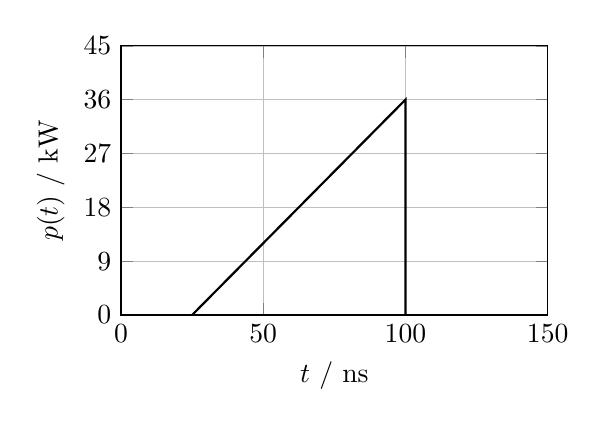
\begin{tikzpicture}
                \begin{axis}[
                    width=7cm, height=5cm,
                    grid=both,
                    major grid style={line width=.2pt,draw=gray!50},
                    minor grid style={line width=.1pt,draw=gray!20},
                    xlabel={$t$ / ns},
                    ylabel={$p(t)$ / kW},
                    xmin=0, xmax=150,
                    ymin=0, ymax=45,
                    xtick={0, 50, 100, 150},
                    ytick={0,9, 18, 27, 36, 45},
                ]
                % Einschaltverhalten graph
                \addplot[
                    thick,
                    mark=none,
                    color=black,
                ] coordinates {
                    (25,0) (100, 36) (100, 0)
                };
                \end{axis}
            \end{tikzpicture}
            \caption{Power values for the switch-on process.}
            \label{fig:Power values for the switch-on process}
        \end{subfigure}
        \hfill % Abstand zwischen den Subfiguren
        \begin{subfigure}[t]{0.45\textwidth}
            \centering
            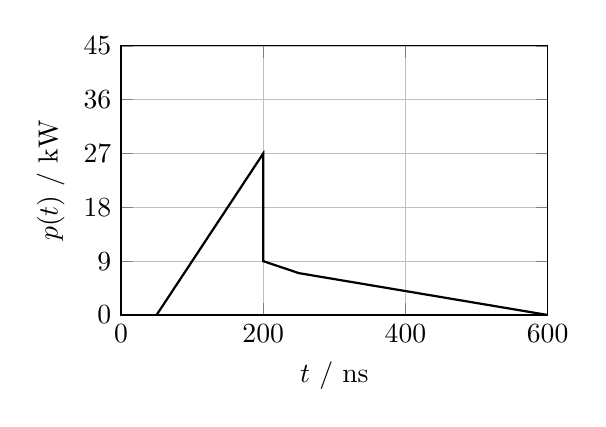
\begin{tikzpicture}
                \begin{axis}[
                    width=7cm, height=5cm,
                    grid=both,
                    major grid style={line width=.2pt,draw=gray!50},
                    minor grid style={line width=.1pt,draw=gray!20},
                    xlabel={$t$ / ns},
                    ylabel={$p(t)$ / kW},
                    xmin=0, xmax=600,
                    ymin=0, ymax=45,
                    xtick={0,200, 400, 600},
                    ytick={0,9, 18, 27,36, 45},
                ]
                % Ausschaltverhalten graph
                \addplot[
                    thick,
                    mark=none,
                    color=black,
                ] coordinates {
                    (50,0) (200, 27) (200, 9) (250, 7) (600,0)
                };
                \end{axis}
            \end{tikzpicture}
            \caption{Power values for the switch-off process.}
            \label{fig:Power values for the switch-off process}
        \end{subfigure}
        \caption{Switch-on behavior and switch-off behavior of $p(t)$}
    \end{solutionfigure}
}